\section{提案する理論}

\subsection{数式}

数式による記述が必要な場合は,式番号を適切に参照しながらまとめること.

\subsection{図・写真}

読者の理解を助けるため,図や表を効果的に利用すること.図のキャプションは

\begin{figure}
    \centering
    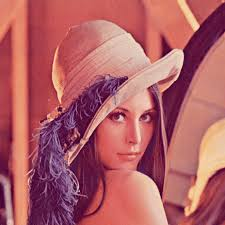
\includegraphics[width=5cm]{figures/Lena.png}
    \caption{This is the most fomous lady. The original image is noode photo.}
\end{figure}

のように,図の下に記す.表のキャプションは

\begin{center}表1 ○○○○\end{center}

のように,表の上に記す.